% !TeX encoding = UTF-8
\documentclass[12pt,A4paper,titlepage]{article}
\usepackage[spanish]{babel}
\usepackage[utf8]{inputenc} %Este paquete permite poner acentos directamente y ees
\usepackage[T1]{fontenc}
\usepackage{amsmath}
\usepackage{graphicx}%[pdftex]
\usepackage{graphicx, wrapfig}
\usepackage{fancyhdr}
\usepackage{anysize}
\usepackage{verbatim}
\usepackage[dvips,final]{epsfig}
\usepackage{epstopdf}
\usepackage{colortbl}
\usepackage{listings}
\usepackage{float}
\usepackage{color}
\marginsize{2.5cm}{2.5cm}{2.5cm}{2.5cm}
\usepackage{fancyhdr}
\pagestyle{fancy}
\fancyhf{}
\fancyhead[LO]{Arquitectura de Computadoras}
\fancyfoot[LE,RO]{\thepage}
\fancyfoot[LO]{Aagaard Martín - Navarro Matias}
\renewcommand{\footrulewidth}{0.4pt}


%\graphicspath{{figuras/}}

%defiino un estilo de ingreso de codigo
\definecolor{codegreen}{rgb}{0,0.6,0}
\definecolor{codegray}{rgb}{0.5,0.5,0.5}
\definecolor{codepurple}{rgb}{0.58,0,0.82}
\definecolor{backcolour}{rgb}{0.95,0.95,0.92}
 
\lstdefinestyle{mystyle}{
    backgroundcolor=\color{backcolour},   
    commentstyle=\color{codegreen},
    keywordstyle=\color{magenta},
    numberstyle=\tiny\color{codegray},
    stringstyle=\color{codepurple},
    basicstyle=\footnotesize,
    breakatwhitespace=false,         
    breaklines=true,                 
    captionpos=b,                    
    keepspaces=true,                 
    numbers=left,                    
    numbersep=5pt,                  
    showspaces=false,                
    showstringspaces=false,
    showtabs=false,                  
    tabsize=2
}
\lstset{style=mystyle}
\setlength{\parindent}{1cm}
\setlength{\parskip}{\baselineskip} 

\begin{document}
\renewcommand{\tablename}{Tabla}
\large

\title{Arquitectura de Computadoras \\
\large Trabajo Páctico Nº1 - Implementación de ALU en HDL}
\author{Aagaard Martin - Navarro Matias\\ Universidad Nacional de Córdoba \bigskip
  \bigskip}

\date{11 de septiembre de 2019}

\begin{titlepage}
\center


\begin{figure}[h]
    \centering
    
\includegraphics[scale=0.8]{figure/logos-fcefyn-y-unc.png}
    \label{fig:unc-logo}
\end{figure}

{\let\newpage\relax\maketitle}
\center
\end{titlepage}

\maketitle % Compila la carátula
\tableofcontents % Arma el índice
\newpage

\section{Introducción}
En toda implementacion de software hay algunos componentes de hardware sumamente necesarios para su funcionamiento. En el siguiente informe se describirá el diseño, la implementacion y el testing de uno de estos elementos: ALU. \\
La  ``ALU'' (Unidad Aritmetica Logica) es un circuito combinacional digital que calcula operaciones aritmeticas asi como operaciones logicas entre argumentos.

\section{Implementación del practico}
Entre los dispositivos disponibles para la Implementación de la ALU se selecciono la placa de desarrollo Basys 3. La principal razón de la selección fue que esta placa es el único modelo disponible y que soporta la interfaz de desarrollo Vivado. La FPGA sobre la que se trabajara es la Artix-7 de Xilinx.

\subsection{Desarrollo del módulo ALU}
Este módulo contiene el desarrollo de las funcionalidades de la ALU, las cuales consisten en un set de operaciones sobre dos registros, y un selector sobre estas que define la salida del módulo.

Es un módulo puramente combinacional, razón por la cual no contiene entrada de \textit{clock} y sus salidas dependen directamente de los cambios en sus entradas. 


La ALU cuenta con tres entradas y una salida, con un ancho de palabra parametrizable y con valores por defecto de 8 bits. 

\begin{figure}[H] 
	\centering
	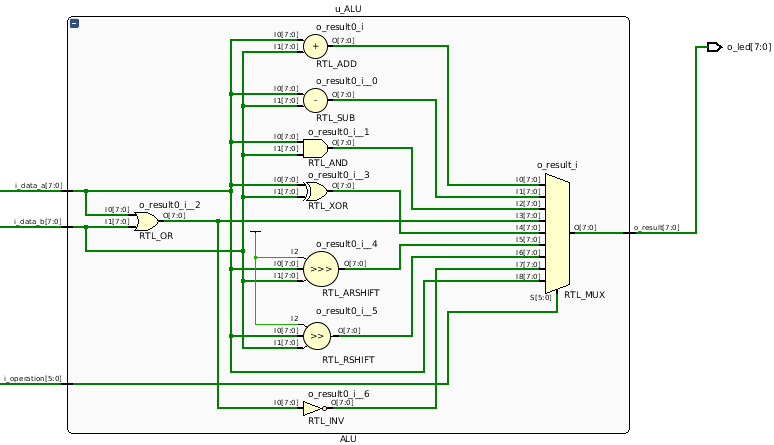
\includegraphics[scale=0.6]{figure/rtl-alu.png}
	\caption{\textit{Estructura RTL del módulo ALU obtenida de la herramienta Verilog}}
\end{figure}

\subsection{Simulaciones del módulo}
Para comprobar el correcto funcionamiento del módulo, se desarrollaron varios test desde la herramienta, donde se puede ver la respuesta de las señales a diferentes estímulos.

\begin{itemize}
	\item Simulación de la operación de suma: Se simula incrementando los operandos A y B en cada ciclo de clock para comprobar varios resultados. 
	
	\begin{figure}[H] 
		\centering
		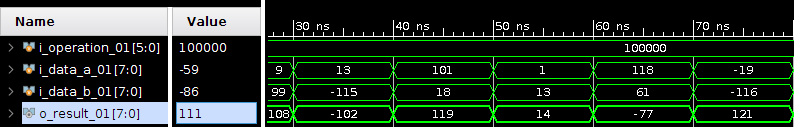
\includegraphics[scale=0.6]{figure/test-suma.png}
		\caption{\textit{Simulación de la operación de suma}}
	\end{figure}
	\item Simulación de operación AND: Se incrementa el operando A y decrementa B en el test en cada ciclo de clock para obtener diferentes resultados
	
	\begin{figure}[H] 
		\centering
		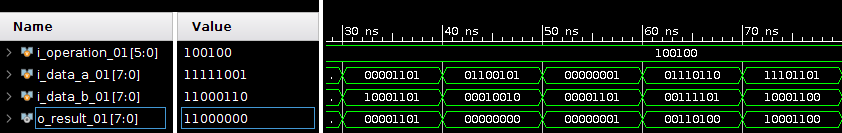
\includegraphics[scale=0.6]{figure/test-and.png}
		\caption{\textit{Simulación de la operación AND}}
	\end{figure}

\end{itemize}


\subsection{Implementación en FPGA}
Para la implementación se instancia el módulo ALU dentro de un módulo top, sobre el cual se declaran como entradas y salidas los pines de la FPGA a utilizar. 

Para mapear los pines de la FPGA con las entradas y salidas del módulo, se importo un recurso llamado \textbf{\textit{constraints}}, el cual consiste en un archivo con extensión xdc correspondiente a la placa de desarrollo a utilizar. En el archivo de \textbf{\textit{constraints}} se encuentran todas las lineas comentadas y se le deben sacar los comentarios a las que se van a utilizar como E/S en el módulo top. En nuestro proyecto de utilizaron las siguientes E/S:
\begin{itemize}
	\item i\_clk (Clock 100 MHz)
	\item i\_sw[7:0] para entradas
	\item i\_btn [2:0] para seleccionar las entradas
\end{itemize}

Para evitar latches en este módulo se trabajó con una señal de clock, la cual es encargada de sincronizar las entradas al módulo ALU y la carga de los registros sobre los cuales esta va operar. 

\begin{figure}[H] 
	\centering
	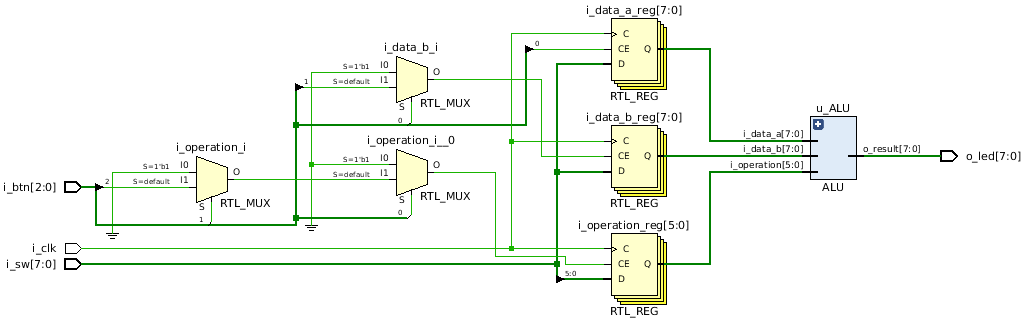
\includegraphics[scale=0.55]{figure/rtl-top.png}
	\caption{\textit{Estructura RTL del módulo top obtenida de la herramienta Verilog}}
\end{figure}

\newpage
\section{Conclusión}
Mediante un desarrollo sencillo de una ALU, se pudo comprender el principio de funcionamiento de una FPGA. Una vez terminado el práctico, a través de la herramienta Verilog se obtuvieron las especificaciones de la utilización del la FPGA en términos de LUT y FF como se introdujo en clase 

\begin{figure}[H] 
	\centering
	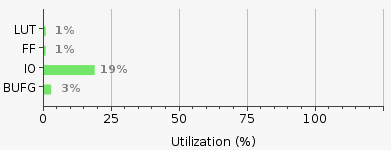
\includegraphics[scale=0.7]{figure/utilizacion.png}
	\caption{\textit{Utilización de la FPGA}}
\end{figure}

\end{document}

